% Preamble
\documentclass[12pt]{article}

% Packages
\usepackage[left=3.0cm, right=1.5cm, top=2.0cm, bottom=2.0cm]{geometry}

\usepackage[utf8]{inputenc}
\usepackage[T2A]{fontenc}
\usepackage[russian]{babel}
\usepackage{amsmath, amsfonts, amssymb}
\usepackage{graphicx}
\usepackage{wrapfig}
\usepackage{fancyhdr}
\usepackage[shortlabels]{enumitem}
\usepackage{svg}
\usepackage{amstex}
\usepackage{colortbl}
\usepackage{bm}

\renewcommand{\vec}{\textbf}
\newcommand{\cross}{\times}

\pagestyle{fancy}
\fancyhead[L]{Работа №4.7.3}
\fancyhead[R]{Белинский Т.Д.\quad Б05-206}

% Document
\begin{document}
    \section*{4.7.3. ПОЛЯРИЗАЦИЯ}
    \ \par
    \textbf{Цель работы:} ознакомление с методами получения и анализа поляризованного света.

    \textbf{Оборудование:} оптическая скамья с осветителем; зелёный светофильтр; два поляроида; чёрное зеркало;
    полированная эбонитовая пластинка; стопа стеклянных пластинок; слюдяные пластинки разной толщины;
    пластинки в 1/4 и 1/2 длины волны; пластинка в одну длину волны для зелёного света
    (пластинка чувствительного оттенка).


    \subsection*{Теоретическая часть}
    \ \par
    \textbf{Получение эллиптически поляризованного света.}
    Эллиптически поляризованный свет можно получить из линейно поляризованного с
    помощью двоякопреломляющих кристаллических пластинок.

    Двоякопреломляющая пластинка имеет два взаимно перпендикулярных главных направления,
    совпадающих с осями эллипсоида диэлектрической проницаемости.
    Волны, поляризованные вдоль главных направлений, распространяются в пластинке с разными
    скоростями, не изменяя характера своей поляризации.
    Эти волны называются главными.
    Мы будем обозначать показатели преломления для главных волн через $n_x$ и $n_y$,
    где $x$ и $y$ -- главные направления кристаллической пластинки.
    Пусть на пластинку падает линейно поляризованная волна,
    электрический вектор которой ориентирован под некоторым углом $\alpha$ к оси $x$.
    Разложим вектор $E$ на составляющие $E_x$ и $E_y$.
    На входе пластинки $E_x$ и $E_y$ находятся в фазе.
    На выходе из-за разности скоростей между ними появляется разность хода $d(n_x − n_y)$,
    при этом сдвиг фаз определяется соотношением:
    \begin{equation}
        \Delta \varphi = \frac{2\pi}{m} = kd(n_x - n_y),
        \label{eq:1}
    \end{equation}
    где $k$ — волновое число (в пустоте), $d$ — толщина кристаллической пластинки.
    Как уже отмечалось, при сложении двух взаимно перпендикулярных колебаний,
    обладающих некоторым сдвигом фаз, образуется колебание, поляризованное по эллипсу.

    Рассмотрим практически важные частные случаи.
    \begin{enumerate}
        [a)]
        \item Пластинка даёт сдвиг фаз $2\pi$ (пластинка в длину волны $\lambda$).
        В результате сложения волн на выходе пластинки образуется
        линейно поляризованная волна с тем же направлением колебаний, что и в падающей волне.
        \item Пластинка даёт сдвиг фаз $π$ (пластинка в полдлины волны $\lambda/2$).
        На выходе пластинки снова образуется линейно поляризованная волна.
        Направление $bb'$ колебаний этой волны повёрнуто относительно направления $aa'$ колебаний падающей волны.
        Как нетрудно сообразить, направление $bb'$ является зеркальным отображением направления $aa'$
        относительно одного из главных направлений пластинки.
        Такую пластинку используют для поворота направления колебаний линейно поляризованного света.
        \item Пластинка создаёт между колебаниями сдвиг фаз $\pi/2$ (пластинка в четверть длины волны).
        При сложении двух взаимно перпендикулярных колебаний, имеющих разность фаз $\pi/2$, образуется эллипс, главные
        оси которого совпадают с координатными осями $x$ и $y$.
        При равенстве амплитуд $E^{max}_x = E{^max}_y$ возникает круговая поляризация.
    \end{enumerate}

    Следует отметить, что, говоря о пластинках $\lambda$, $\lambda/2$, $\lambda/4$ и т. д.,
    всегда подразумевают какую-либо вполне определённую монохроматическую компоненту
    (например, пластинка $\lambda/2$ для зелёного света).
    Если на двоякопреломляющую пластинку падает не монохроматический свет, то на
    выходе из неё для разных спектральных компонент эллипсы поляризации будут различными.

    \textbf{Анализ эллиптически поляризованного света.}
    Анализ эллиптически поляризованного света сводится к нахождению главных осей
    эллипса поляризации и к определению направления вращения электрического вектора.
    Главные оси эллипса поляризации определяются с помощью анализатора по максимуму и минимуму интенсивности проходящего света.
    Направление вращения электрического вектора может быть найдено с помощью пластинки в четверть длины волны, для которой известно,
    какая из главных волн, $E_x$ или $E_y$, имеет большую скорость распространения (и соответственно меньшее значение показателя преломления).

    Выберем для определённости координатные оси $x$ и $y$ на пластинке так, чтобы $n_x$ < $n_y$.
    В этом случае главная волна $E_x$ имеет большую скорость распространения.
    Поместим такую пластинку на пути эллиптически поляризованного света
    и совместим главные направления пластинки $\lambda/4$ с главными осями эллипса поляризации.
    На выходе из этой пластинки сдвиг фаз между $E_x$ и $E_y$ вместо $\pi/2$ станет равным нулю или $\pi$.
    Свет окажется линейно поляризованным. Из двух возможных значений сдвига фаз, $0$ или $\pi$,
    реализуется одно: то, которое соответствует имеющемуся в волне направлению вращения электрического вектора.

    Рассмотрим, например, случай, когда электрический вектор в эллиптически поляризованной волне вращается против часовой стрелки,
    если смотреть навстречу лучу.
    В этом случае, очевидно, в волне, падающей на пластинку в $\lambda/4$, колебание $E_y$ отстаёт по фазе на $\pi/2$ от
    колебания $E_x$.
    При прохождении через пластинку разность фаз увеличивается до $\pi$. Таким образом на выходе из пластинки возникают
    линейно поляризованные волны со сдвигом фаз $\pi$.
    Сложение этих волн даёт плоскополяризованную волну,
    электрический вектор которой располагается во втором и четвёртом квадрантах координатной системы $x$, $y$.

    Рассуждая аналогичным образом, найдём, что при вращении электрического вектора по часовой стрелке
    направление колебаний в линейно поляризованной волне, выходящей из пластинки,
    располагается в первом и третьем квадрантах.
    Определяя направление колебаний на выходе из пластинки с помощью поляроида,
    можно, таким образом, определить характер эллиптической поляризации (вращение против или по часовой стрелке).

    \textbf{Пластинка чувствительного оттенка.}
    Выше предполагалось известным, какому из двух главных направлений пластинки в четверть
    длины волны соответствует большая скорость распространения света.
    Установить это можно различными способами, например с помощью
    пластинки чувствительного оттенка (так называют пластинку в $\lambda$
    для зелёной спектральной компоненты, $\lambda = 560$ нм).

    Пластинка имеет форму стрелы, вдоль оси которой расположено главное направление, соответствующее большей скорости распространения.

    Если пластинка чувствительного оттенка помещена между скрещенными поляроидами и главные направления пластинки не параллельны
    направлениям разрешённых колебаний поляроидов, то при освещении белым светом пластинка кажется окрашенной в лилово-красный цвет.
    Это объясняется тем, что зелёная компонента линейно поляризованного света при прохождении пластинки
    не меняет поляризации и задерживается вторым поляроидом.
    Для красной и фиолетовой компонент пластинка создаёт сдвиг фаз, несколько отличный от $2\pi$.
    На выходе из пластинки красная и фиолетовая компоненты оказываются
    поэтому эллиптически поляризованными и частично проходят через второй поляроид.
    Таким образом, в известном смысле наблюдаемый в указанном опыте цвет пластинки дополнителен к зелёному.

    Если между скрещенными поляроидами поместить пластинку чувствительного оттенка
    ($\lambda$) и пластинку в $\lambda/4$ так, чтобы их главные направления совпадали, цвет пластинки изменится.
    Если у пластинки чувствительного оттенка и пластинки в $\lambda/4$ совпадут главные направления, соответствующие большей скорости
    распространения, то разность хода между $E_x$ и $E_y$ для зелёного света составит уже $5\lambda/4$.
    Это соответствует разности хода в $\lambda$ для света с большей длиной волны, т. е. для «более красного» света.
    При освещении этих пластинок (напомним, что они расположены между скрещенными поляроидами) белым светом теперь погасится не зелёная, а красная
    часть спектра, и проходящий свет будет казаться зеленовато-голубым.
    Если же главные направления, соответствующие большей скорости распространения, у пластинки чувствительного оттенка и у пластинки
    в $\lambda/4$ окажутся перпендикулярными, то проходящий свет приобретёт
    оранжево-желтую окраску (погасится фиолетово-голубая часть спектра).

    Изменение цвета позволяет, таким образом, определить, какое из
    главных направлений пластинки в $\lambda/4$ соответствует большей скорости
    распространения.

    \textbf{Интерференция поляризованных лучей.}
    Тонкие двоякопреломляющие пластинки, помещённые между поляроидами, кажутся окрашенными.
    Эта окраска может быть истолкована как результат интерференции поляризованных лучей.
    Здесь $p_1p'_1$ -- разрешённое направление колебаний поляризатора (первого поляроида);
    $x$, $y$ -- координатная система, связанная с главными направлениями двоякопреломляющей пластинки;
    $p_2p'_2$ -- разрешённое направление колебаний анализатора (второго поляроида).
    Волны $E_x$ и $E_y$ на выходе из пластинки когерентны, но не могут интерферировать, так как $E_x \perp E_y$.
    Волны $E_1$ и $E_2$ на выходе второго поляроида также являются когерентными и к тому же поляризованы в одной плоскости.
    Эти волны интерферируют между собой.
    Результат интерференции определяется зависящим от длины волны сдвигом фаз между $E_1$ и $E_2$.
    В результате интерференции поляризованных лучей пластинка, освещаемая белым светом, кажется окрашенной.

    Если поворачивать двоякопреломляющую пластинку, расположенную между
    скрещенными поляроидами, то соотношение амплитуд волн $E_1$ и $E_2$ и разность фаз между ними не изменяются.
    Это означает, что цвет пластинки при её поворотах не меняется, а меняется только интенсивность света.
    За один оборот пластинки интенсивность четыре раза обращается в нуль -- это происходит при совпадении главных направлений
    $x$ и $y$ с разрешёнными направлениями колебаний поляроидов.
    Если же двоякопреломляющую пластинку оставить неподвижной, а второй поляроид повернуть так, чтобы разрешённые направления
    $p_1p'_1$ и $p_2p'_2$ совпали, то волны $E_1$ и $E_2$ приобретают дополнительный фазовый сдвиг на $\pi$
    для всех спектральных компонент;
    при этом их амплитуды изменятся так, что цвет пластинки изменится на дополнительный.
    Студентам предлагается самостоятельно это доказать

    \subsection*{Результаты и обработка}
    \begin{enumerate}
        \item \textbf{Определение разрешенных направлений поляроида.}
        Методом последовательных приближений (поворачиваем зеркало и поляроид) была получена минимальная интенсивность
        (черное пятно) при отражении от зеркала света, прошедшего через поляроид.
        Отсчет по лимбу для поляроида P1 $(82.6\pm0.2) ^{\circ}$.
        \begin{table}[h!]
            \centering
            \caption{Запись по лимбу для разрешенного направления поляроида P1}
            \label{tab:1}
            \begin{tabular}{|l|ccccc|}
                \hline
                №                     & 1  & 2  & 3  & 4  & 5  \\\hline
                $\varphi$, $^{\circ}$ & 83 & 82 & 82 & 83 & 83 \\
                \hline
            \end{tabular}
        \end{table}

        Скрестив первый поляроид со вторы получили минимум интенсивности при отсчете по лимбу P2 $(-9.8\pm 0.2)^{\circ}$.
        \begin{table}[h!]
            \centering
            \caption{Запись по лимбу для разрешенного направления поляроида P2}
            \label{tab:2}
            \begin{tabular}{|l|ccccc|}
                \hline
                №                     & 1  & 2   & 3   & 4   & 5   \\\hline
                $\varphi$, $^{\circ}$ & -9 & -10 & -10 & -10 & -10 \\
                \hline
            \end{tabular}
        \end{table}

        \item \textbf{Определение показателя преломления для эбонита.}
        Поворачивая зеркало, ищем минимум интенсивности отраженного света прошедшего через поляроид.
        Начало отсчета $(88.0\pm0.5)^{\circ}$ -- зеркало выставлено параллельно поляроиду.

        \begin{table}[h!]
            \centering
            \caption{Запись по лимбу зеркала для минимума интенсивности}
            \label{tab:3}
            \begin{tabular}{|l|ccccc|}
                \hline
                №                     & 1  & 2  & 3  & 4  & 5  \\\hline
                $\varphi$, $^{\circ}$ & 31 & 31 & 32 & 33 & 32 \\
                \hline
            \end{tabular}
        \end{table}

        \begin{table}[h!]
            \centering
            \caption{Запись по лимбу зеркала для минимума интенсивности зеленого света}
            \label{tab:4}
            \begin{tabular}{|l|ccccc|}
                \hline
                №                     & 1  & 2  & 3  & 4  & 5  \\\hline
                $\varphi$, $^{\circ}$ & 32 & 33 & 32 & 33 & 32 \\
                \hline
            \end{tabular}
        \end{table}

        Итоговые значения: $(56\pm1)^{\circ}$, зеленый свет: $(56\pm1)^{\circ}$.
        Показатель преломления оценим по формуле $n = \tan \varphi_{\text{Б}}$.
        \[
            n = (1.49 \pm 0.03) \quad n_{\text{з}} = (1.46 \pm 0.03)
        \]


        \item \textbf{Исследование поляризации света в преломленном и отраженном от стопы лучах.}
        Освещаем стопу неполяризованным светом и рассматриваем через поляроиды отраженный от стопы и преломленный лучи.
        Результаты представлены в таблице.
        \begin{table}[h!]
            \centering
            \caption{Поляризация света в преломленном и отраженном от стопы лучах}
            \label{tab:5}
            \begin{tabular}{|l|cc|}
                \hline
                & Вертикальная поляризация & Горизонтальная поляризация \\\hline
                Преломленный свет & $-$                      & $+$                        \\
                Отраженный свет   & $+$                      & $-$                        \\
                \hline
            \end{tabular}
        \end{table}

        \item \textbf{Определение главных направлений двоякопреломляющих пластин.}
        Вращая пластинку вокруг направления луча и наблюдая за интенсивностью света,
        проходящего сквозь второй поляроид, определяем, положение при котором
        интенсивность света минимальна -- при этом условии главные направления пластинки совпадают с
        разрешёнными направлениями поляроидов.
        Полученные отсчеты по лимбу для пластин:
        \[
            \varphi_{\lambda/2} = (5\pm1)^{\circ}\quad
            \varphi_{\lambda/4} = (62\pm1)^{\circ}.
        \]
        \item \textbf{Выделение пластин /2 и /4.}
        Устанавливаем разрешённое направление первого поляроида горизонтально, а главные направления исследуемой пластинки —
        под углом $45^{\circ}$ к горизонтали.
        Наблюдаем свет через второй поляроид, вращая его:
        \begin{itemize}
            \item[$\lambda/4$] ничего не меняется -- поляризация круговая;
            \item[$\lambda/4$] минимумы сменяют максимумы и т.д -- линейная поляризация.
        \end{itemize}

        \item \textbf{Определение быстрой и медленной оси в пластине}
        Определите «быструю» и «медленную» оси в пластинке $\lambda/4$:
        Поставим между скрещенными поляроидами пластинку чувствительного оттенка, имеющую вид стрелки.
        Из первого поляроида выходит горизонтально поляризованный свет, второй пропускает -- вертикально поляризованный.
        Добавляем к схеме пластинку $\lambda/2$, главные оси повернуты под углом $45^{\circ}$ к горизонту.
        При повороте рейтера со стрелкой на 180◦ вокруг вертикальной оси цвет стрелки меняется от зелёно-голубого до оранжево-жёлтого.
        В случае когда цвет стрелки зелено-голубой -- ее направление совпадает с быстрой осью пластины $\lambda/2$.

        \item \textbf{Интерференция поляризованных лучей}
        Расположим между скрещенными поляроидами мозаичную слюдяную пластинку.
        Она собрана из 4-х узких полосок слюды, лежащих по сторонам квадрата
        (две полоски «толщиной» $\lambda/4$ и по одной -- $\lambda/2$ и $3\lambda/4$).
        В центральном квадратике слюды нет.
        Главные направления всех пластинок ориентированы параллельно сторонам квадрата.
        Вращая пластинку, наблюдаются изменения интенсивностей в отдельных квадратиках.
        Не трогая пластинки, вращаем поляроид, при этом цвета квадратиков изменяются на дополнительные.
        Чем отличается эффект?
        Опишите и объясните результат.

        \item \textbf{Направление вращения светового вектора в эллиптически
        поляризованной волне.}

        \begin{minipage}[h!]{0.48\linewidth}
            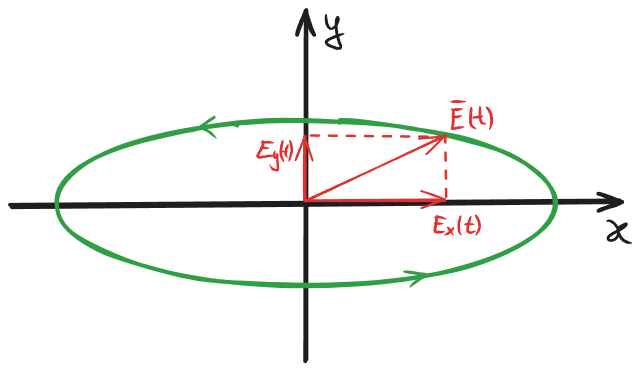
\includegraphics[width=\linewidth]{pic/elips}
            \caption{Рис. 1: Эллипс поляризации вектора $\textbf{E}$}
        \end{minipage}
        \hfill
        \begin{minipage}[h!]{0.48\linewidth}
            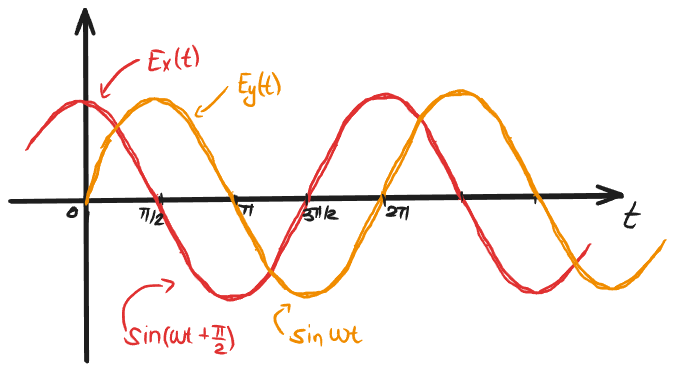
\includegraphics[width=\linewidth]{pic/sin}
            \caption{Рис. 2: Графики зависимости $E_x, E_y$ от времени}
        \end{minipage}

        Нетрудно заметить, что направление вращения вектора $\textbf{E}$ против часовой стрелки возникает
        при разнице фаз $\varphi_x - \varphi_y = \pi/2$.
        Вращению по часовой стрелке соответствует $\varphi_x - \varphi_y = -\pi/2$.
        Если быстрая ось -- $Ox$, то разность фаз $-\varphi_x + \varphi_y = kd(n_x - n_y) < 0$,
        то есть вектор $\textbf{E}$ после пластинки $\lambda/4$ вращается против часовой стрелке.
        Устанавливаем разрешённое направление первого поляроида под углом $\sim 15^{\circ}$ к горизонтали.
        Устанавливаем разрешённое направление второго поляроида вертикально, вращая пластинку,
        находим минимальную интенсивность света, прошедшего второй поляроид.
        Так мы получили эллипс поляризации с вертикально ориентированной малой осью.

        Устанавливаем между поляроидами дополнительную пластинку $\lambda/4$ с горизонтально ориентированной «быстрой» осью.
        В этом случае свет на выходе из второй пластинки будет линейно поляризован.
        При этом световой вектор перешел в смежные квадранты, то есть пластинки дают эллипсы, вращающиеся в одну сторону.
        Значит направление вращение против часовой стрелке.
    \end{enumerate}
\end{document}